\documentclass[12pt, %larger font size
			  t     %frames are top-aligned
]{beamer}%
\mode<presentation>

\usetheme{Garching}

\usepackage[utf8]{inputenc}
\usepackage[english,ngerman]{babel}%
\usepackage[autostyle=true]{csquotes}%
\usepackage{graphicx}
\usepackage[export]{adjustbox} % to align images
\usepackage{booktabs}
\usepackage{multimedia} % for /media to embed videos

\makeatletter
\setbeamertemplate{footline}{
  \leavevmode%
  \hbox{%
  \begin{beamercolorbox}[wd=\paperwidth,ht=2.25ex,dp=2ex,left]{author in head/foot}%
    \usebeamerfont{author in head/foot}%\insertshortauthor
    \hskip 12.05cm
    \insertframenumber{}
  \end{beamercolorbox}}
}
\makeatother


\title{Dynamical Post-Processing\\ for Manipulation Trajectories}%
\subtitle{Internship Report}%
\author{Sarah Braun}%
\institute[TU München]{Technische Universität München}%
\titlegraphic{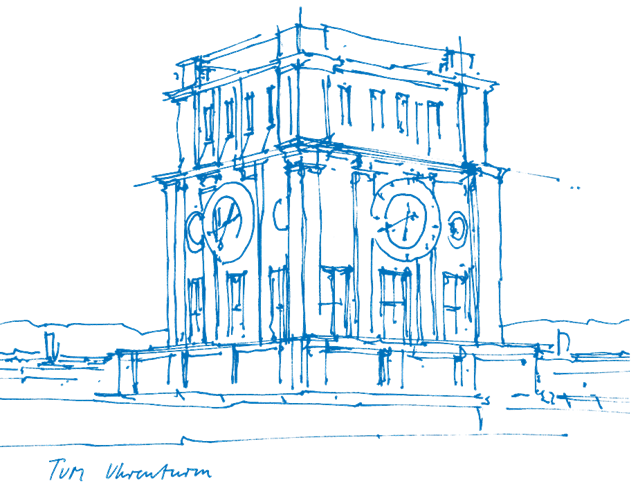
\includegraphics[height=0.3\paperheight]{tum-uhrenturm}}
\date{July 24th, 2017}%


\begin{document}
\selectlanguage{english}

%------TITLEFRAME-----------------------------------------------------------------------
\begin{frame}[plain]
  \titlepage
\end{frame}

%------MOTIVATION-----------------------------------------------------------------------
\begin{frame}
\frametitle{Motivation}
\begin{itemize}
\item sampling-based manipulation planners output kinematic path
\item dynamics not yet taken into account
\item local improvements possible
\end{itemize}
\end{frame}



%-------POST-PROCESSING STRATEGIES--------------------------------------------------
\begin{frame}
  \frametitle{Evaluation of Various Post-Processing Strategies}
  \begin{enumerate}
  \item Hauser's shortcutting idea
  \item Smooth object interaction
  \item Sampling of new transitions
  \item \textcolor{gray}{Sampling of new grasps and placements}
  \end{enumerate}
\end{frame}

%-------HAUSER SHORTCUTTING-------------------------------------------------------------
\begin{frame}
 \frametitle{1. Hauser's Shortcutting Idea}

 \begin{columns}[T]
   \begin{column}{.5\textwidth}
     \begin{itemize}
     \item \only<1>{sample two points} \only<2->{\textcolor{gray}{sample two points}}
     \item\only<1>{compute shortcut}\only<2->{compute shortcut \textcolor{orange}{How?}}
     \item \only<1>{check collisions} \only<2->{\textcolor{gray}{check collisions}}
     \end{itemize}
   \end{column}
   
   \begin{column}{.5\textwidth}
     \includegraphics[height=0.6\paperheight, right]{../Images/Hauser_Shortcutting.pdf}
   \end{column}
 \end{columns}
\end{frame}

%-------SYNCHRONIZATION OF AXES-------------------------------------------------------------
\begin{frame}
\frametitle{Synchronization of Axes}
\vskip -.3cm
\begin{columns}[T]
  \begin{column}{.5\textwidth}
    \begin{block}{Basic Idea}
      \begin{itemize}
        \item find "bottleneck" axis
	    \item synchronize all axes to bottleneck time
	  \end{itemize}
	\end{block}
  \end{column}

  \only<-2>{
  \begin{column}{.5\textwidth}
    \invisible{
    \begin{block}{Reflexxes}
      \begin{itemize}
        \item find "bottleneck axis" and inoperative time intervals
        \item synchronize all axes to earliest possible point in time
      \end{itemize}
    \end{block}}
  \end{column}
  }

  \only<3>{
  \begin{column}{.5\textwidth}
    \begin{block}{Reflexxes}
      \begin{itemize}
        \item find "bottleneck axis" and inoperative time intervals
        \item synchronize all axes to earliest possible point in time
      \end{itemize}
    \end{block}
  \end{column}
  }
\end{columns}

\vskip -1cm
\hskip -.57cm
\only<2>{
\textbf{\textcolor{orange}{Problem}}
\setlength{\leftmargini}{.4cm}
\begin{itemize}
  \item  synchronization to arbitrary subsequent point in time not always possible
  \item each axis has inoperative time intervals in which axis cannot be synchronized
  \end{itemize}
}

\end{frame}

%-------SMOOTH INTERACTION---INITIAL STATE--------------------------------------------
\begin{frame}
\frametitle{2. Smooth Interaction}
  \begin{itemize}
    \item "interaction" = approaching the object to be gripped
  \end{itemize}

  \centering
    \fbox{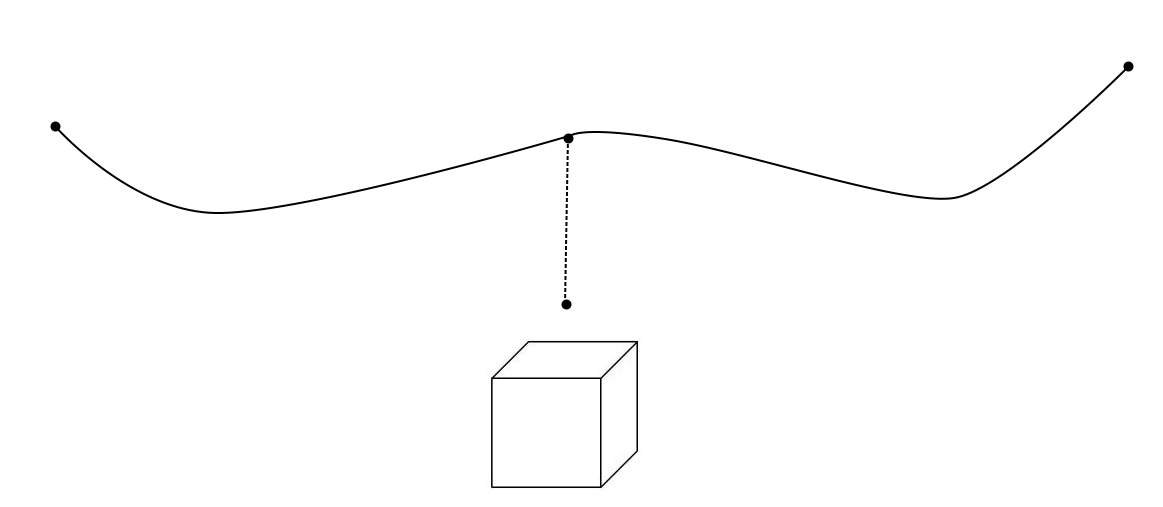
\includegraphics[scale=0.2]{../Images/SmoothInteraction_smaller.jpg}}
    \begin{itemize}
      \item stopping takes a lot of time\\
      \invisible{test}
    \end{itemize} 
\end{frame}


%-------SMOOTH INTERACTION---BETTER-------------------------------------------------
\begin{frame}
\frametitle{2. Smooth Interaction}
  \begin{itemize}
    \item "interaction" = approaching the object to be gripped
  \end{itemize}
  
  \centering
  \fbox{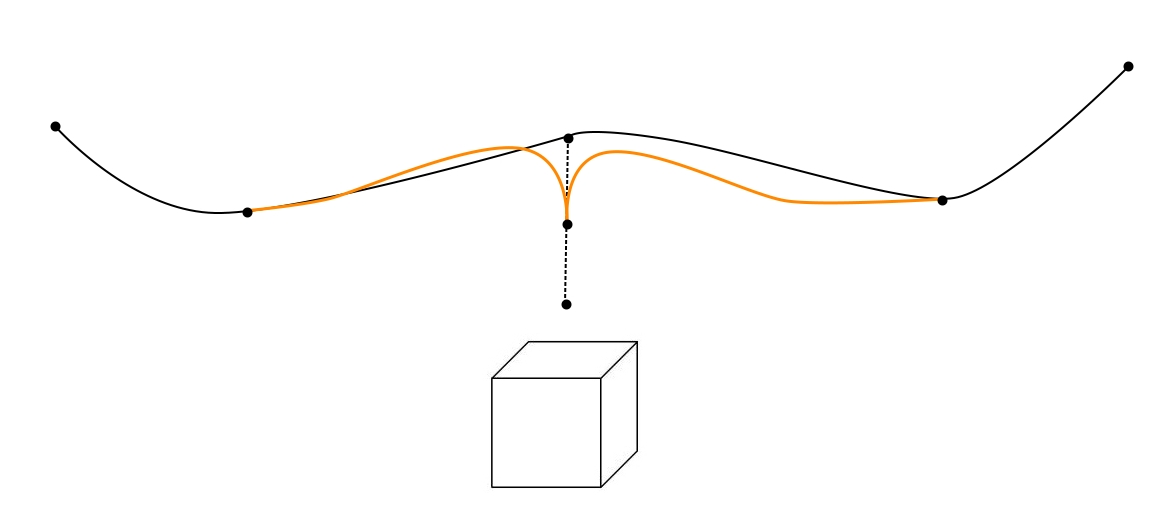
\includegraphics[scale=0.2]{../Images/SmoothInteraction_smaller_orange_2.jpg}}
  \begin{itemize}
    \item better: slide smoothly into linear movement
    \item use Reflexxes for computation of orange motion
  \end{itemize}
\end{frame}

%-------TRANSITION SAMPLING---BASIC IDEA-----------------------------------------------
\begin{frame}
\frametitle{3. Sampling of New Transitions - Basic Idea}
\begin{itemize}
  \item Recall: Manipulation Planner\\ 
        \textcolor{red}{PHILIPP'S IMAGE}
  \item Idea: Sample new transitions and re-plan trajectories in adjacent modes
\end{itemize}


\end{frame}

%-------TRANSITION SAMPLING---MORE DETAILS-----------------------------------------------
\begin{frame}
\frametitle{3. Sampling of New Transitions - More Details}
\begin{itemize}
  \item new transition is ... 
  \begin{columns}[T]
    \begin{column}{.05\textwidth}
    \end{column}
    \begin{column}{.475\textwidth}
       \footnotesize{... either new inverse kinematic} \\ \vskip 0.3cm
       \centering \fbox{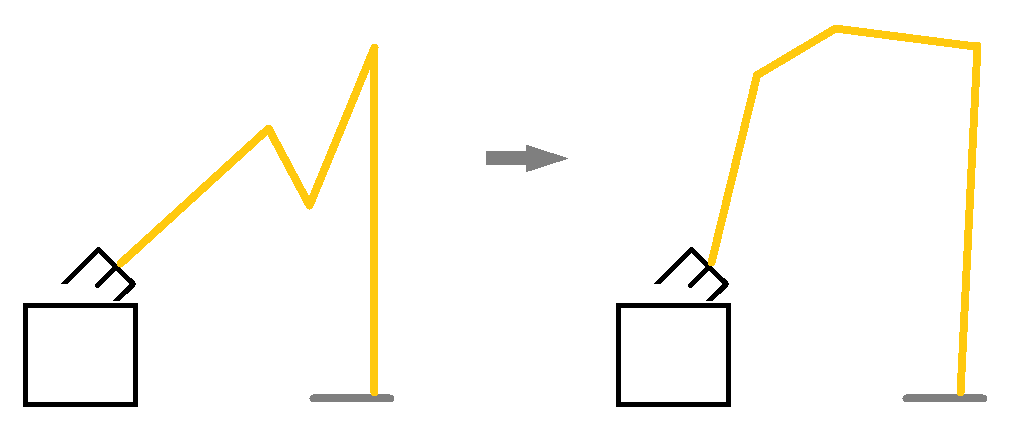
\includegraphics[scale=0.08]{../Images/New_Transition.png}}
    \end{column}
    \begin{column}{.475\textwidth}
      \footnotesize{... or arbitrary valid configuration} \\ \vskip 0.24cm                                                                            
      \hskip -.13cm \fbox{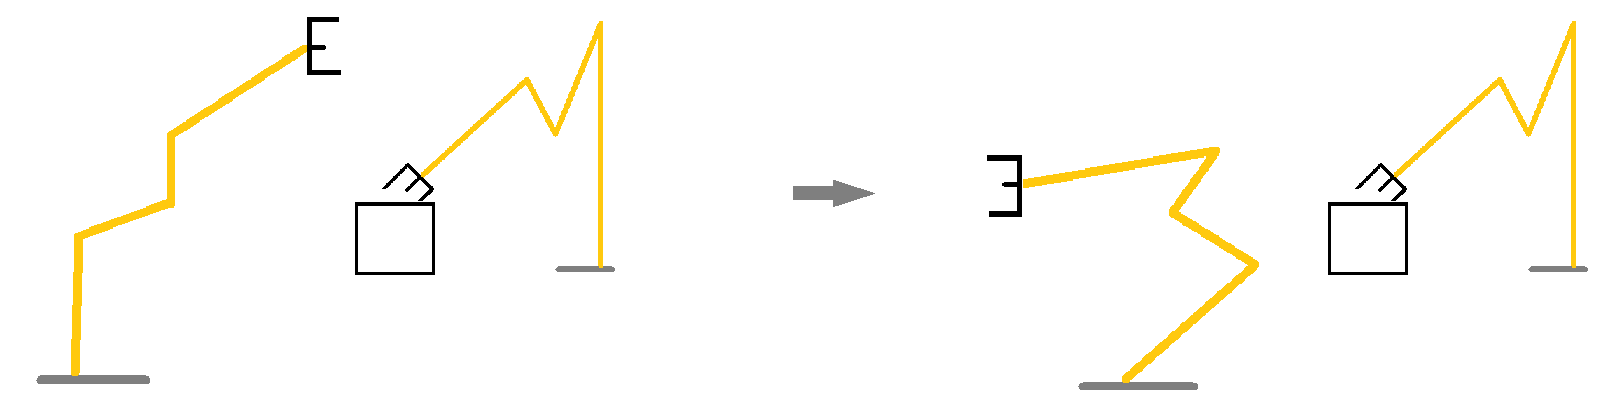
\includegraphics[scale=0.112]{../Images/New_Transition_4.png}}
    \end{column}
  \end{columns} 
  \vskip .3cm  
  \item Replan using Reflexxes:\\ \textcolor{red}{include picture similar to Philipp's}
  % two manifolds, transition area, new transition in different color, sampled point and Reflexxes' connection also in different color
% Im_3
\end{itemize}


\end{frame}

%-------GRASP SAMPLING--------------------------------------------------------------
\begin{frame}
\frametitle{4. Sampling of New Grasps and Placements}
\begin{itemize}
  \item Recall: Within-contact roadmaps for a couple of \textit{fixed} grasps and placements
  \item Idea: Also sample new grasps and replan
  \item Difficulties: new grasp changes planning scene for all subsequent modes, expensive updates
  % Bild von Philipp mit roadmap of roadmaps, streiche hier eine roadmap durch und ersetze sie durch eine neue, zu neuem Grasp gehörend
\end{itemize}


\end{frame}

%-------EVALUATION---BEFORE PP-----------------------------------------------------
\begin{frame}
\label{Plot_Step1}
\frametitle{Evaluation}
\vskip -.3cm
Simple pick-and-place task ... \textcolor{orange}{without} Post-Processing
\begin{center}
  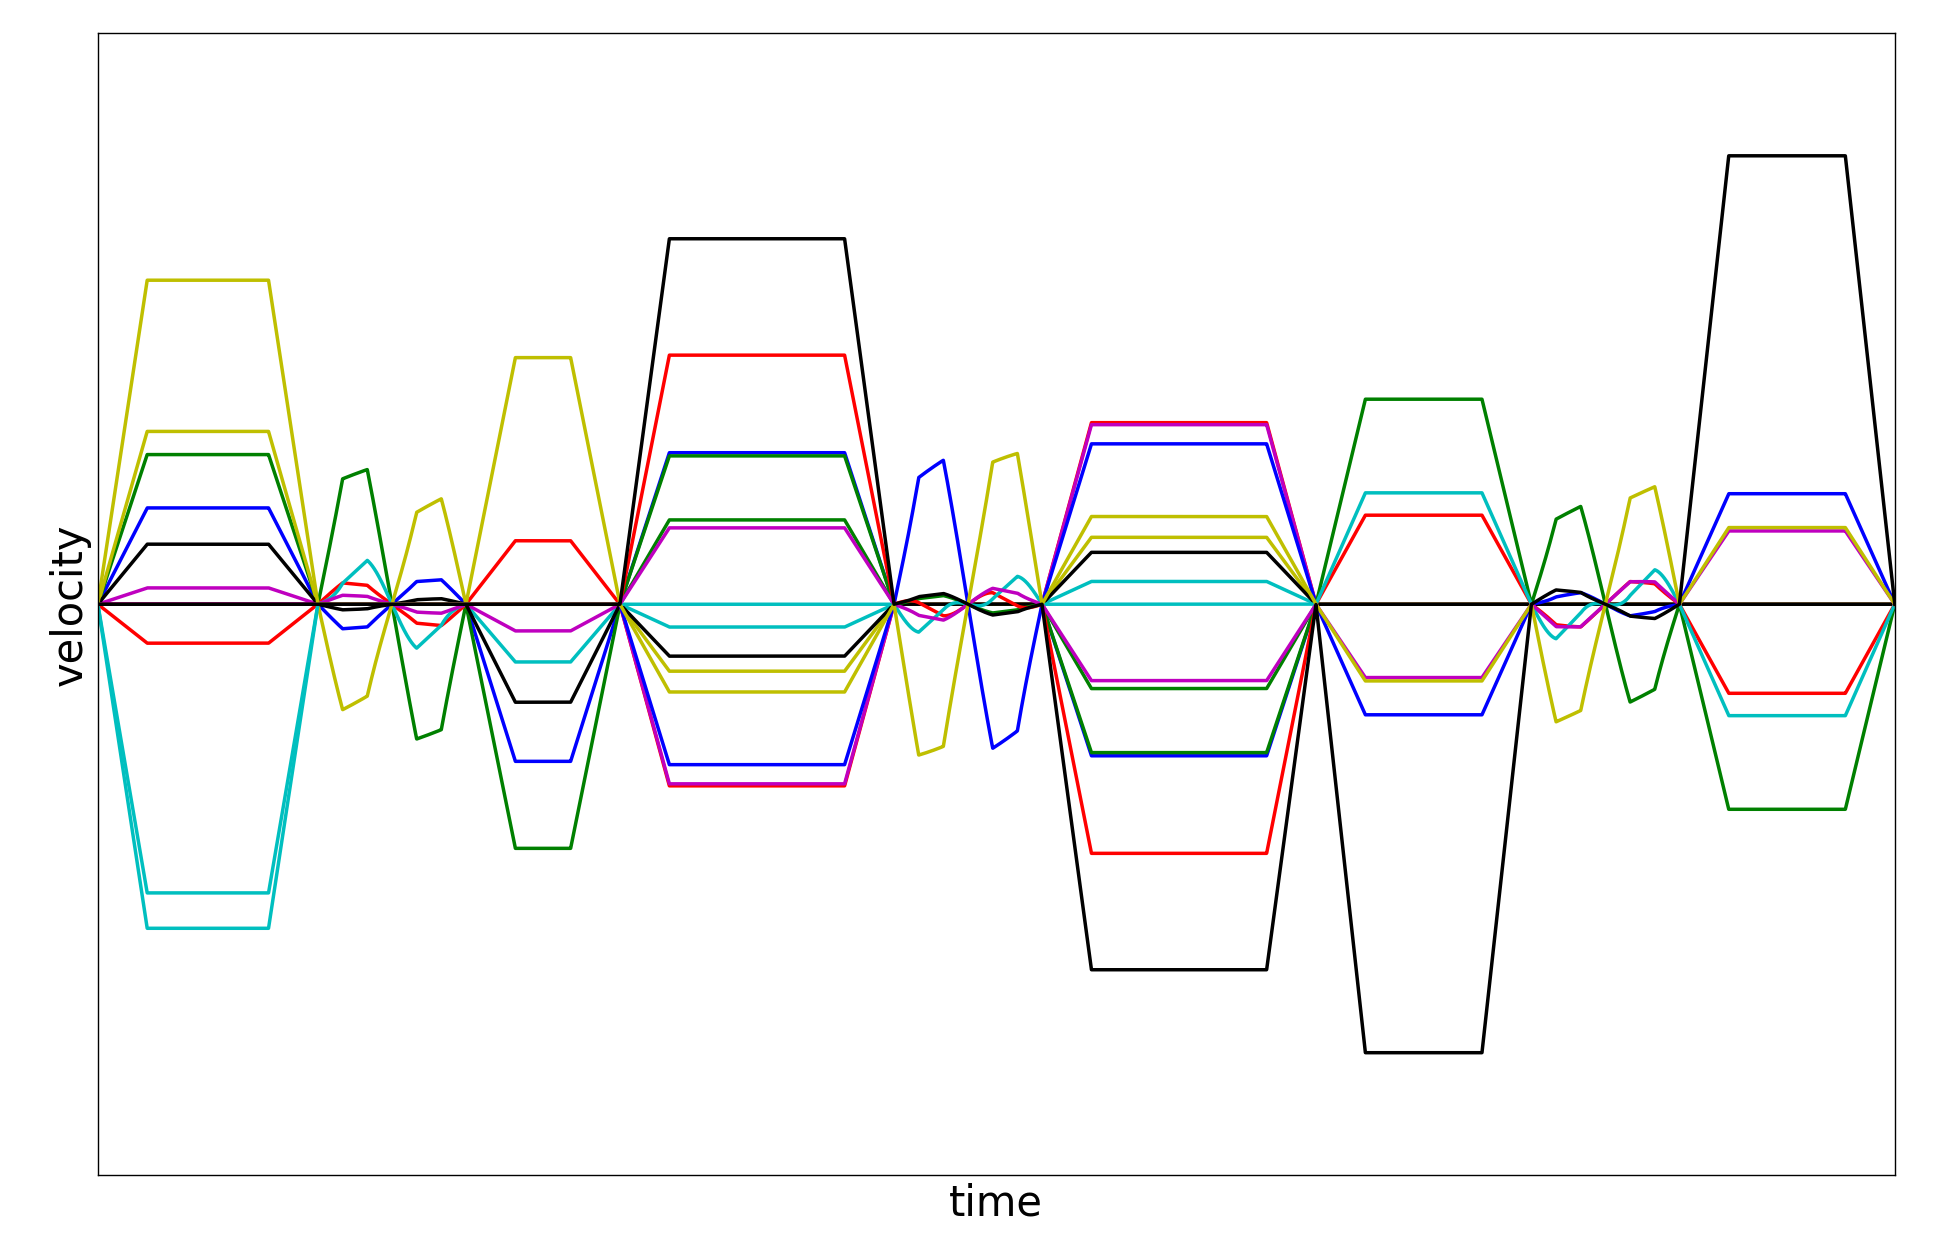
\includegraphics[scale=0.13]{../RecordsAndPlots/Step1.png}
\end{center}
\end{frame}

%-------EVALUATION---AFTER HAUSER--------------------------------------------------
\begin{frame}
\label{Plot_Step2}
\frametitle{Evaluation}
\vskip -.3cm
\invisible{Simple pick-and-place task} ... \textcolor{orange}{after Hauser's Shortcutting}
\begin{center}
  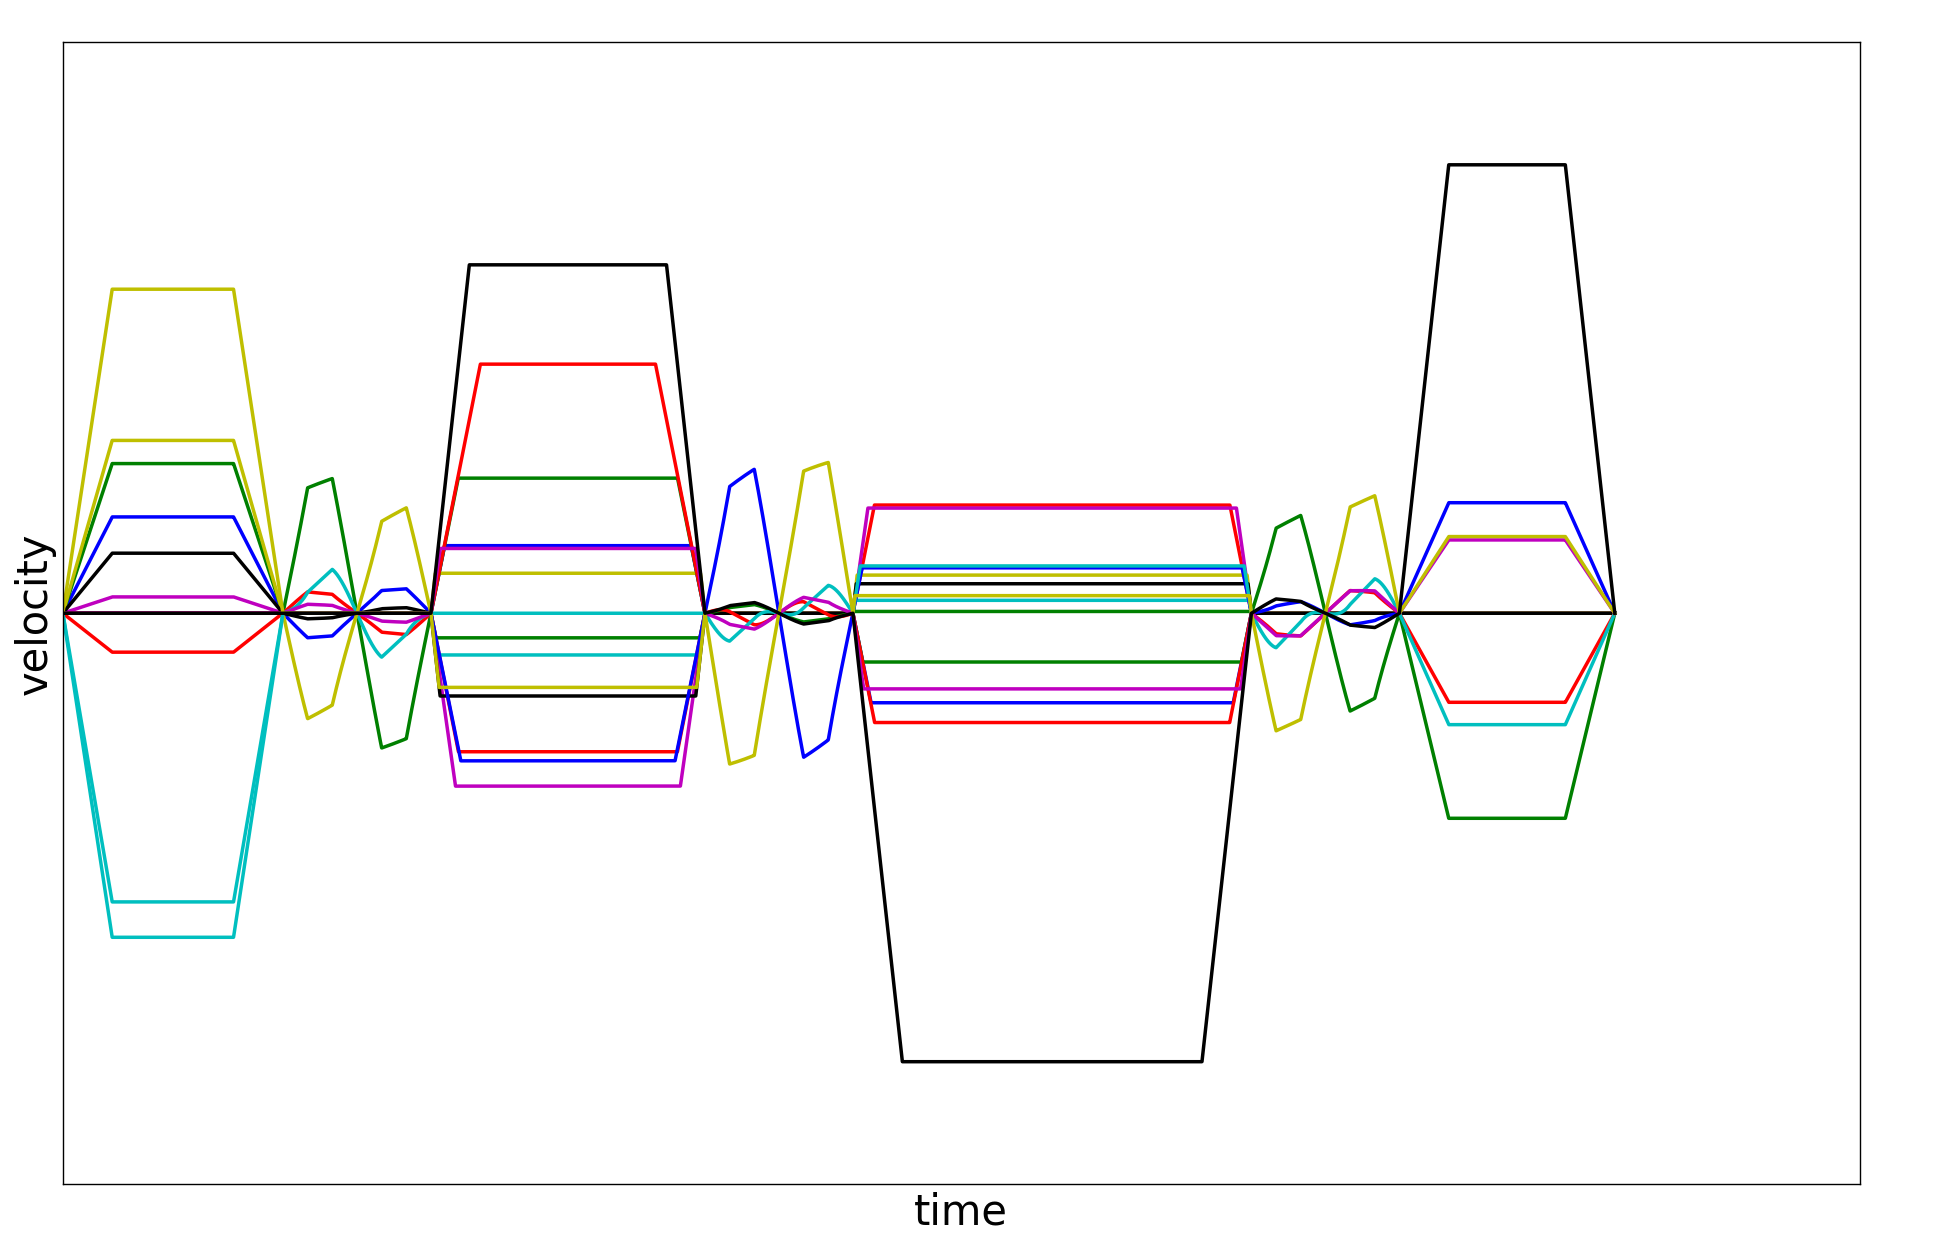
\includegraphics[scale=0.13]{../RecordsAndPlots/Step2.png}
\end{center}
\end{frame}

%-------EVALUATION---AFTER HAUSER + SHORTCUTTING----------------------------------
\begin{frame}
\label{Plot_Step3}
\frametitle{Evaluation}
\vskip -.3cm
\invisible{Simple pick-and-pl} ... \textcolor{orange}{after Shortcutting + Smooth Interaction}
\begin{center}
  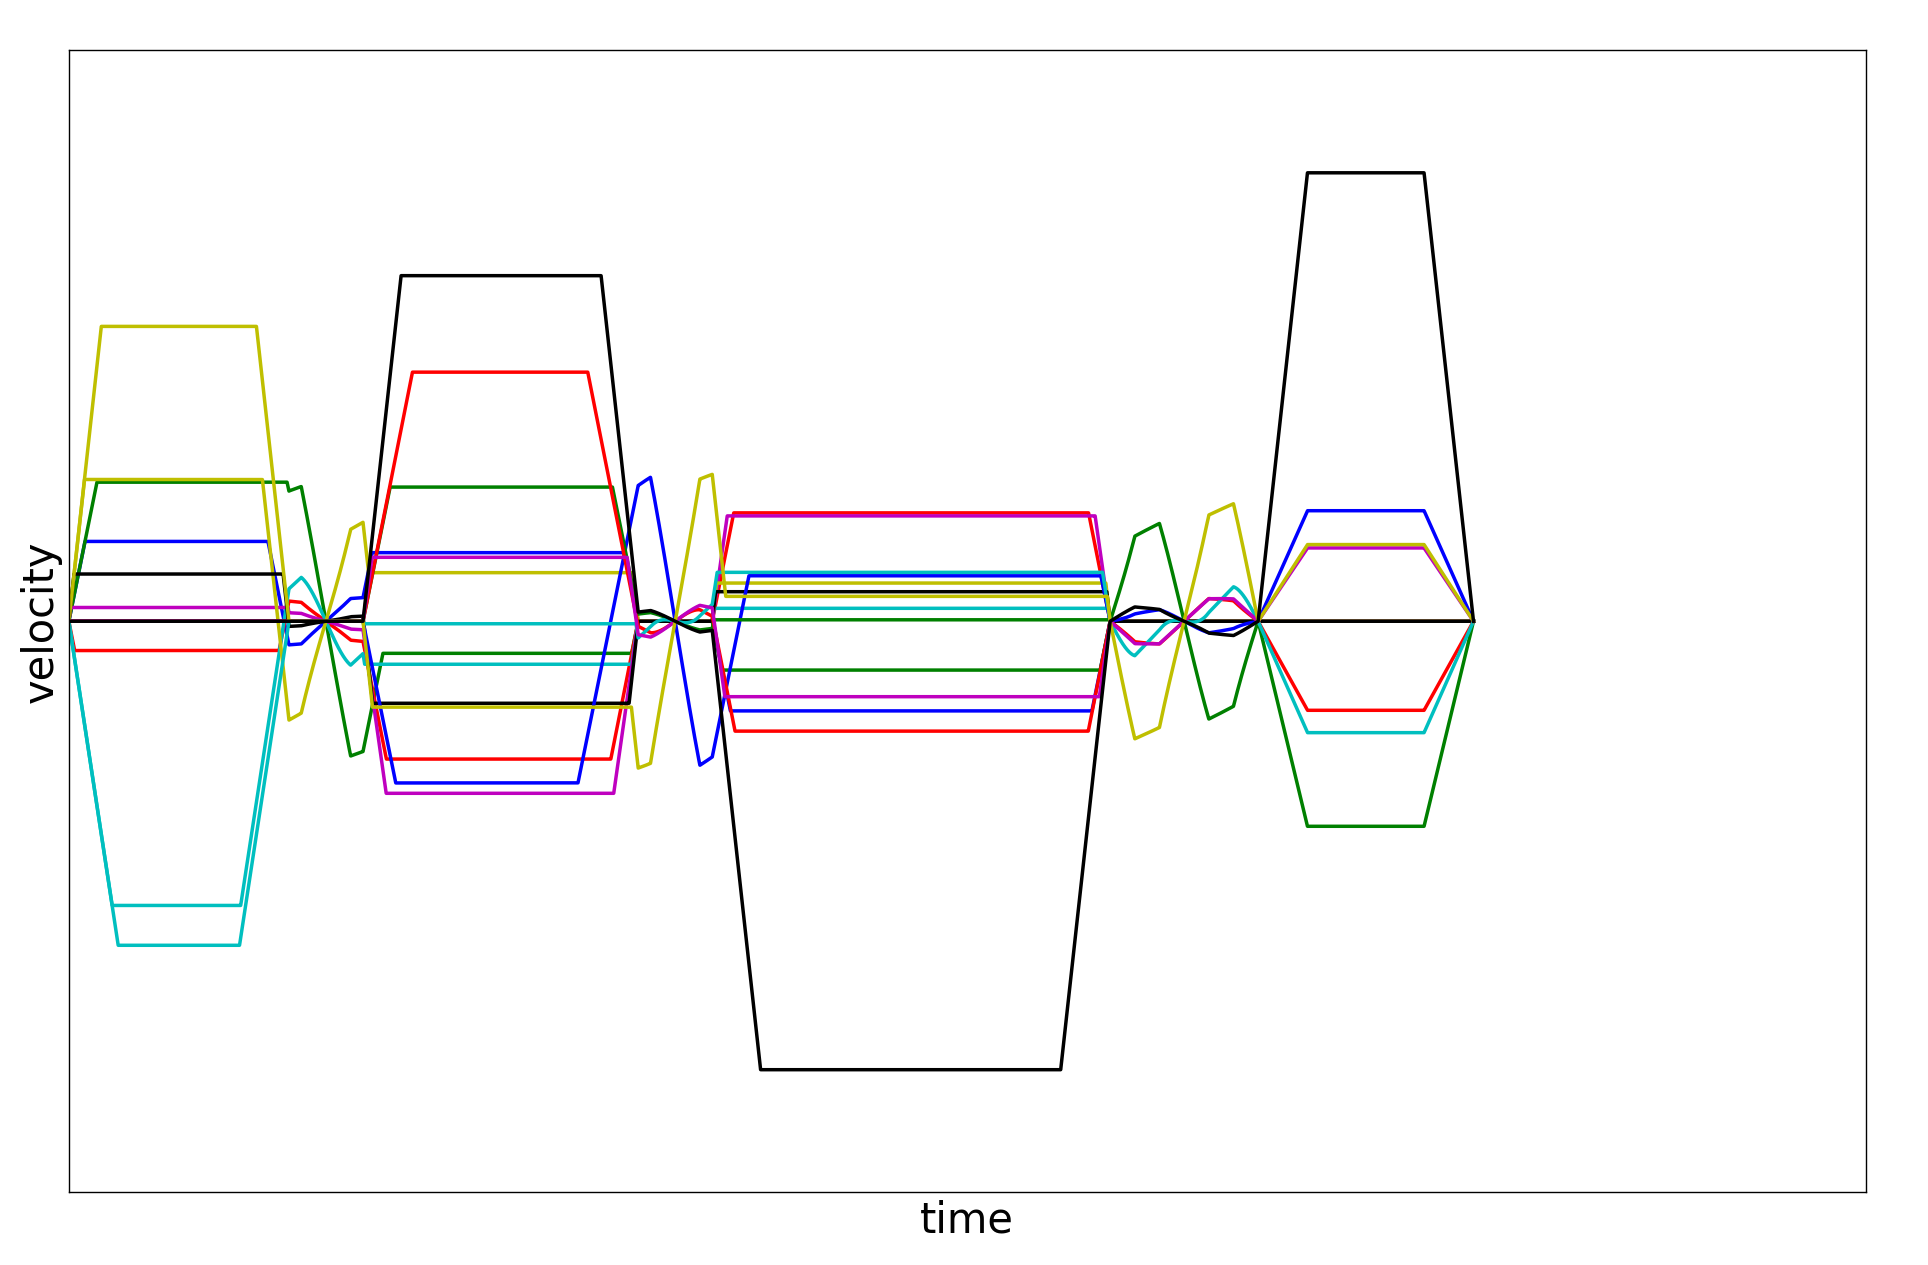
\includegraphics[scale=0.13]{../RecordsAndPlots/Step3.png}
\end{center}
\end{frame}

%-------EVALUATION---AFTER TRANSITION SAMPLING------------------------------------
\begin{frame}
\label{Plot_Step4}
\frametitle{Evaluation}
\vskip -.3cm
\invisible{Simple pick-and-place task} ... \textcolor{orange}{after Transition Sampling}
\begin{center}
  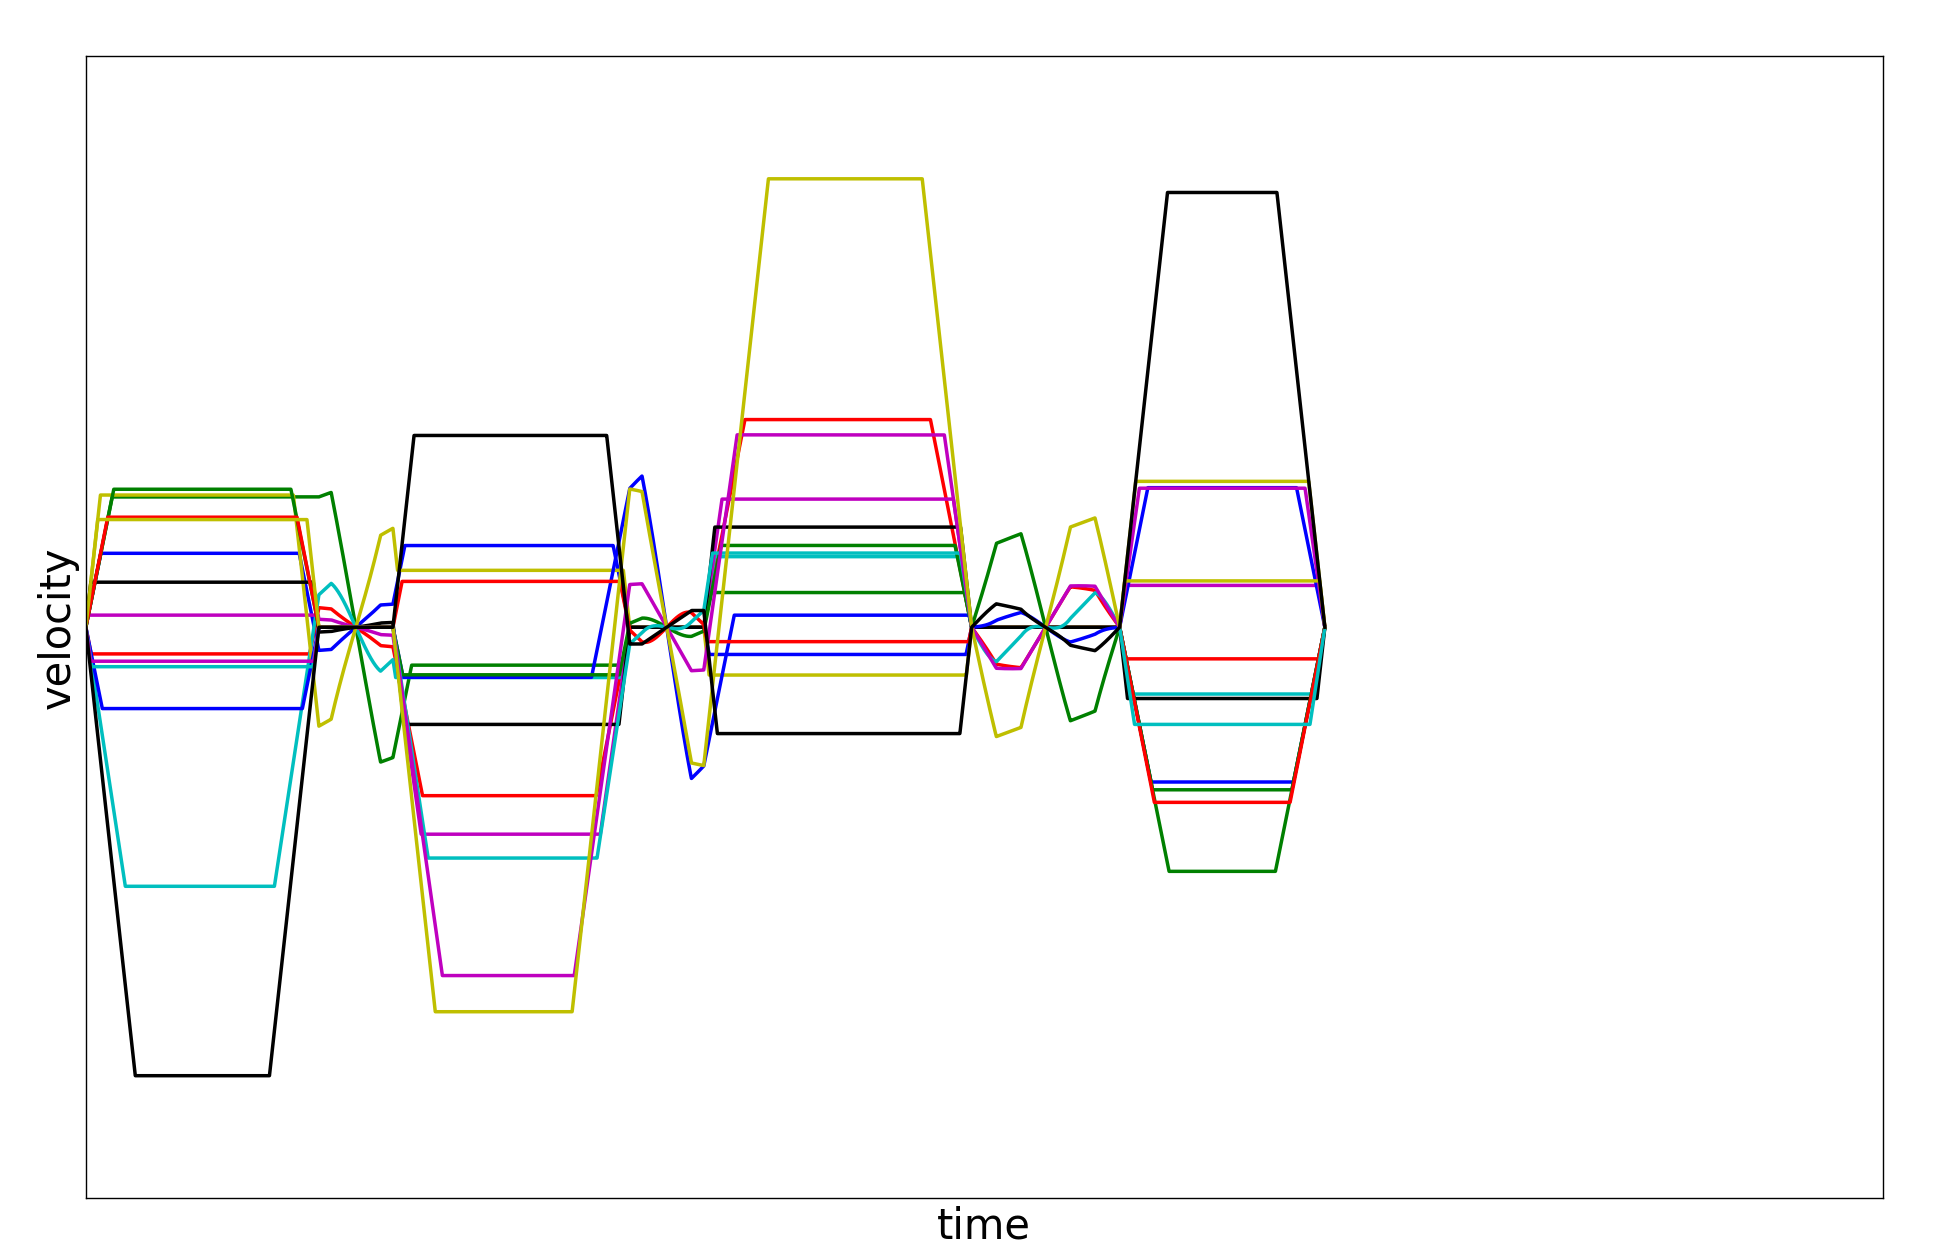
\includegraphics[scale=0.13]{../RecordsAndPlots/Step4.png}
\end{center}
\end{frame}

%-------VIDEO---BEFORE PP-----------------------------------------------------
\begin{frame}
\frametitle{Evaluation}
\vskip -.3cm
Simple pick-and-place task ... \textcolor{orange}{without} Post-Processing
\centering
\movie[height = 6cm, width = 5.4cm, showcontrols, poster]{}{../RecordsAndPlots/Step1.mkv}
\end{frame}


%-------VIDEO---AFTER PP-----------------------------------------------------
\begin{frame}
\frametitle{Evaluation}
\vskip -.3cm
Simple pick-and-place task ... \textcolor{orange}{after} Post-Processing
\centering
\movie[height = 6cm, width = 5.4cm, showcontrols, poster]{}{../RecordsAndPlots/Step4.mkv}
\end{frame}

%-------COMPARISON-----------------------------------------------------
\begin{frame}
\frametitle{Comparison of the Post-Processing Steps}
\centering
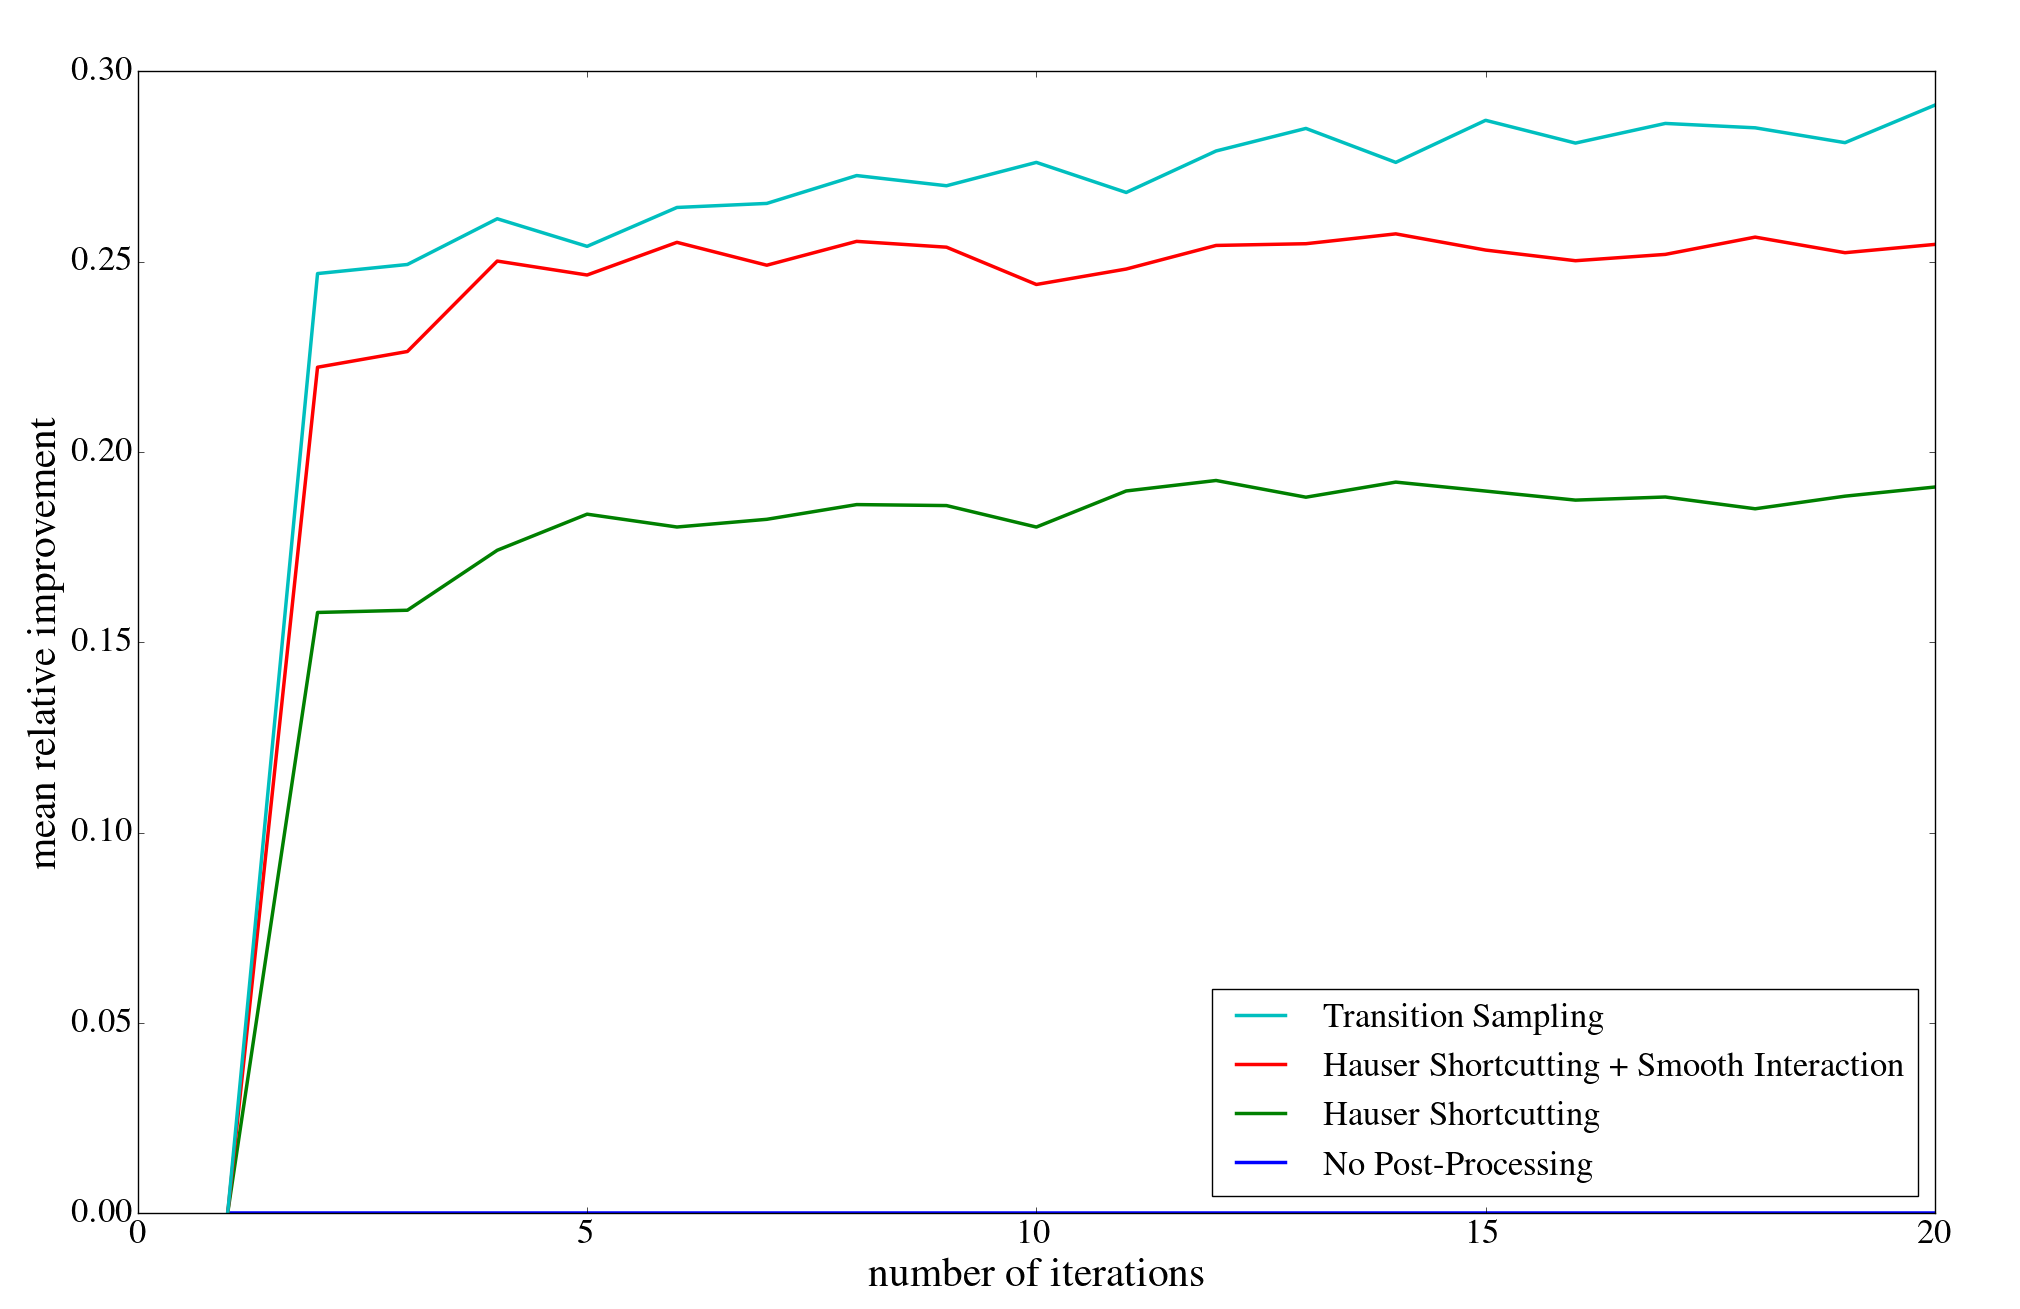
\includegraphics[scale=0.14]{../Images/Comparison.png}
\end{frame}

%-------THESIS-------------------------------------------------------
\begin{frame}
\frametitle{Outlook Master's Thesis}
\begin{columns}[T]
\begin{column}{.55\textwidth}
\small
\begin{itemize}
\item Task: Modeling of a dynamic manipulation task as a MINLP
\item MINLP = \textbf{M}ixed \textbf{I}nteger \textbf{N}onlinear \textbf{P}rogram
\item Include dynamic constraints into optimization
\end{itemize}
\textcolor{orange}{$\Rightarrow$ Time-optimal offline solutions}
\end{column}

\begin{column}{.45\textwidth}
\small
\begin{itemize}
\item Idea: Heuristic for informed search in sampling-based manipulation planner
\end{itemize}
\textcolor{orange}{$\Rightarrow$ More effective sampling strategies}
\end{column}
\end{columns}
\end{frame}


%----------------------------------------------------------------------
%----------BACKUP------------------------------------------------------
%----------------------------------------------------------------------
\begin{frame}
\centering
\begin{beamercolorbox}[wd=\paperwidth,ht=5cm,dp=1ex,center]{tumblue}
\usebeamerfont{frametitle} \textcolor{tumblue}{Backup}
\end{beamercolorbox}
\end{frame}

\begin{frame}
\frametitle{Synchronization not always possible}
\centering
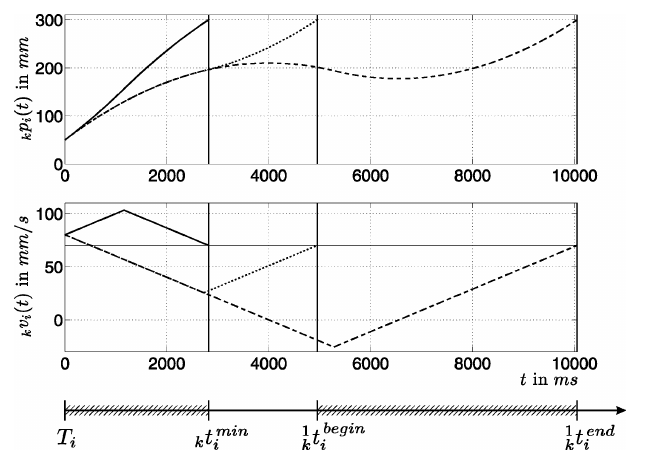
\includegraphics[scale=0.5]{../Images/SynchronizationNotPossible.png}
\end{frame}

\begin{frame}
\frametitle{Synchronization not always possible}
\centering
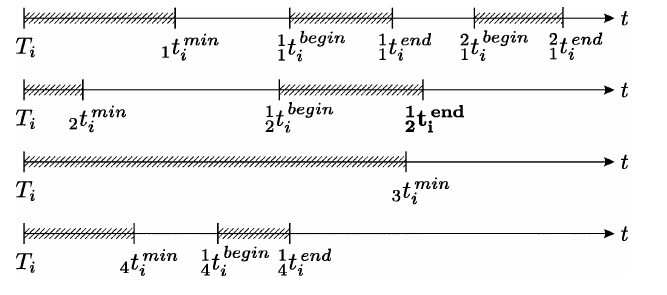
\includegraphics[scale=0.5]{../Images/SynchronizationNotPossible_2.png}
\end{frame}


%----------------------------------------------------------------------
%----------VIDEOS------------------------------------------------------

%----------NO POST-PROCESSING------------------------------------------------------
\begin{frame}
\label{Video_Step1}
\frametitle{No Post-Processing}
\centering
\movie[height = 6cm, width = 5.4cm, showcontrols, poster]{}{../RecordsAndPlots/Step1.mkv}
\hyperlink{Plot_Step1}{\beamerbutton{Plot}}
\end{frame}

%----------HAUSER SHORTCUTTING------------------------------------------------------
\begin{frame}
\label{Video_Step2}
\frametitle{Hauser's Shortcutting}
\centering
\movie[height = 6cm, width = 5.4cm, showcontrols, poster]{}{../RecordsAndPlots/Step2.mkv}
\hyperlink{Plot_Step2}{\beamerbutton{Plot}}
\end{frame}

%----------HAUSER + SMOOTH INTERACTION----------------------------------------------
\begin{frame}
\label{Video_Step3}
\frametitle{Shortcutting plus Smooth Interaction}
\centering
\movie[height = 6cm, width = 5.4cm, showcontrols, poster]{}{../RecordsAndPlots/Step3.mkv}
\hyperlink{Plot_Step3}{\beamerbutton{Plot}}
\end{frame}

%----------TRANSITION SAMPLING-----------------------------------------------------
\begin{frame}
\label{Video_Step4}
\frametitle{Sampling of New Transitions}
\centering
\movie[height = 6cm, width = 5.4cm, showcontrols, poster]{}{../RecordsAndPlots/Step4.mkv}
\hyperlink{Plot_Step4}{\beamerbutton{Plot}}
\end{frame}

\end{document}
